\section*{Unmet need derivation (HNIR52 and HNIR62)}
We derived \texttt{unmet\_need\_c3} for DHS Honduras 2005-06 (HNIR52) and 2011-12 (HNIR62) using a common algorithm aligned with DHS guidance. Women classified as unfecund (menopause/never menstruated/hysterectomy from \texttt{V215}, \texttt{V376==23}, \texttt{V3A08D==1}, or never had sex \texttt{V602==6}) were excluded (NA). Among currently pregnant women (\texttt{V213==1}), pregnancy intention (\texttt{V225}) determined need: wanted then = 0, wanted later = 1 (spacing), not at all = 2 (limiting). Among non-pregnant women who were sexually active (sex in last 30 days; \texttt{V527/V528}, excluding 1 month) or in union (\texttt{V501}), current modern method use (\texttt{V313==3}) was classified as 0. Otherwise, fertility preferences determined need: \texttt{V602==3} = 2 (limiting), \texttt{V602==2} or unknown timing/after marriage = 1 (spacing), and \texttt{V602==1} with preferred wait <2 years = 0 or \textgreater=2 years = 1. All other cases were coded as NA.

\begin{figure}[h!]
\centering
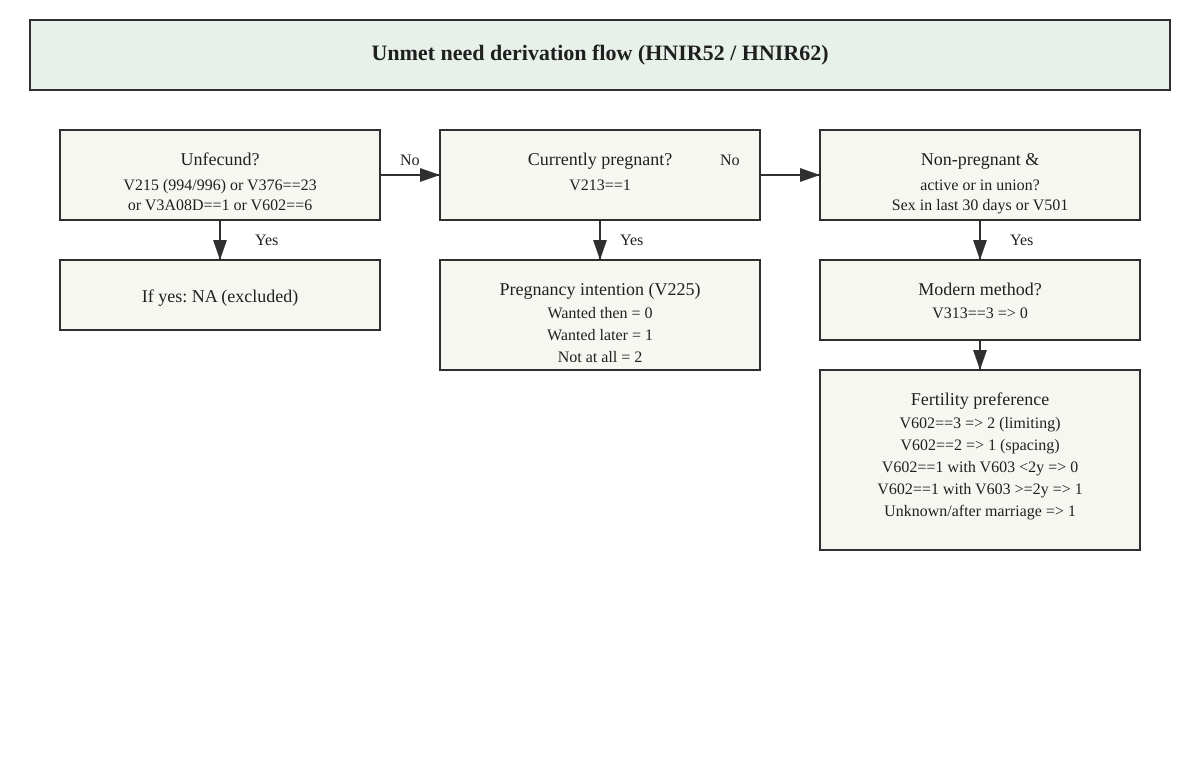
\includegraphics[width=0.95\textwidth]{unmet_need_flowchart.svg}
\caption{Flowchart for \texttt{unmet\_need\_c3} derivation in HNIR52 and HNIR62.}
\end{figure}
